% Asset ID: FA21InequalitiesTikZ-001
% Source: FP1 PDF Ex 4A + teacher transcript
% Related lesson section: Section 9; Worked Example 1
% Purpose: Sketch y=1/x and y=x for 1/x>x.
% Boundary status: Internal portal enrichment, not official CCEA Further Mathematics specification content.
\documentclass[tikz,border=8pt]{standalone}
\usepackage{amsmath}
\usepackage{xcolor}
\definecolor{Canvas}{HTML}{FAF9F6}
\definecolor{Ink}{HTML}{2C2C2E}
\definecolor{LineSoft}{HTML}{E5E5EA}
\definecolor{Gold}{HTML}{C5A059}
\definecolor{WarmPink}{HTML}{FBEFEF}
\begin{document}

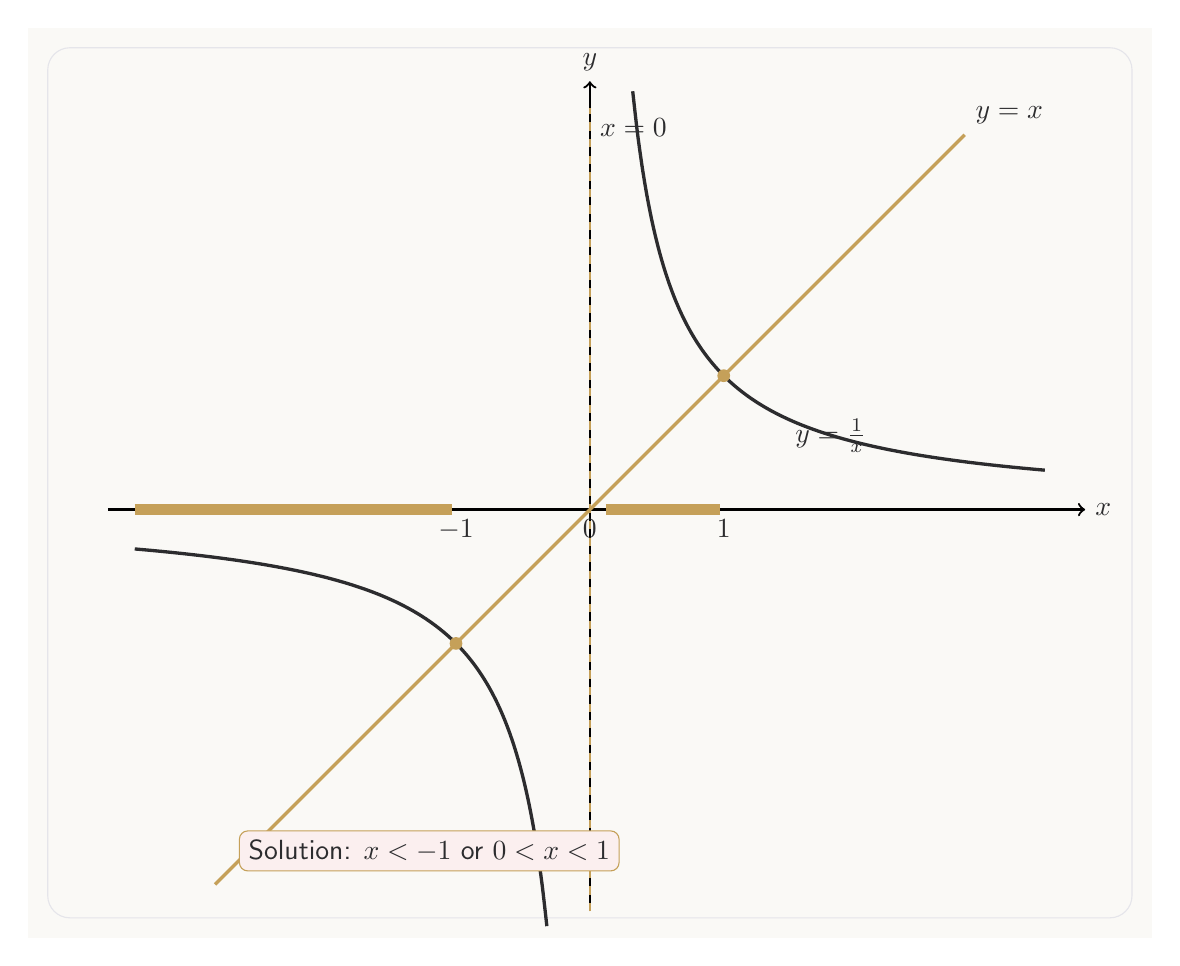
\begin{tikzpicture}[x=1.7cm,y=1.7cm,every node/.style={font=\sffamily,text=Ink}]
\fill[Canvas] (-4.2,-3.2) rectangle (4.2,3.6);
\draw[LineSoft,rounded corners=8pt] (-4.05,-3.05) rectangle (4.05,3.45);
\draw[->,thick] (-3.6,0)--(3.7,0) node[right] {$x$};
\draw[->,thick] (0,-3.0)--(0,3.2) node[above] {$y$};
\draw[Gold,dashed,thick] (0,-3)--(0,3) node[below right] {$x=0$};
\draw[Gold,very thick] (-2.8,-2.8)--(2.8,2.8) node[above right] {$y=x$};
\draw[Ink,very thick,domain=-3.4:-0.32,samples=90,smooth] plot (\x,{1/\x});
\draw[Ink,very thick,domain=0.32:3.4,samples=90,smooth] plot (\x,{1/\x});
\node at (1.8,0.55) {$y=\frac1x$};
\fill[Gold] (-1,-1) circle (2.3pt); \fill[Gold] (1,1) circle (2.3pt);
\draw[Gold,line width=4pt] (-3.4,0)--(-1.03,0);
\draw[Gold,line width=4pt] (0.12,0)--(0.97,0);
\node[below] at (-1,0) {$-1$};\node[below] at (0,0) {$0$};\node[below] at (1,0) {$1$};
\node[fill=WarmPink,draw=Gold,rounded corners=3pt] at (-1.2,-2.55) {Solution: $x<-1$ or $0<x<1$};
\end{tikzpicture}

\end{document}
